\documentclass{article}

% Language setting
% Replace `english' with e.g. `spanish' to change the document language
\usepackage[english]{babel}

% Set page size and margins
% Replace `letterpaper' with`a4paper' for UK/EU standard size
\usepackage[letterpaper,top=2cm,bottom=2cm,left=3cm,right=3cm,marginparwidth=1.75cm]{geometry}

% Useful packages
\usepackage{amsmath}
\usepackage{graphicx}
\usepackage[colorlinks=true, allcolors=blue]{hyperref}

\title{CPE301L: Lab 4}
\author{Joshua Knight, Nicky Victoriano}

\begin{document}
\maketitle
 
\section{Introduction}

In this lab, we are responsible for programming an Arduino similarly to a stoplight. This time, we are only tasked with programming 3 LEDs: red, yellow, and green. Additionally, instead of running automatically like last lab, this time our LEDs are triggered with a button. For an added layer of difficulty, the second part of the lab tasks us with accomplishing these tasks with registry-level programming.

\section{Results}

\subsection{Circuit}

To create our circuit, we set up the ground and power connections between the appropriate rails. Our LEDs were connected by pull-up resistors to the following pins: red to pin 9, yellow to pin 8, and green to pin 7. Our button was connected to pin 10. Then, the Arduino was connected to our computer via the serial port. The final circuit and button configurations can be found in \textbf{Table \ref{tab:light-configs}}.

\begin{table}[]
    \centering
    \begin{tabular}{|c|c|}
         \hline
            \includegraphics[width=0.28\linewidth]{off.jpg} &
            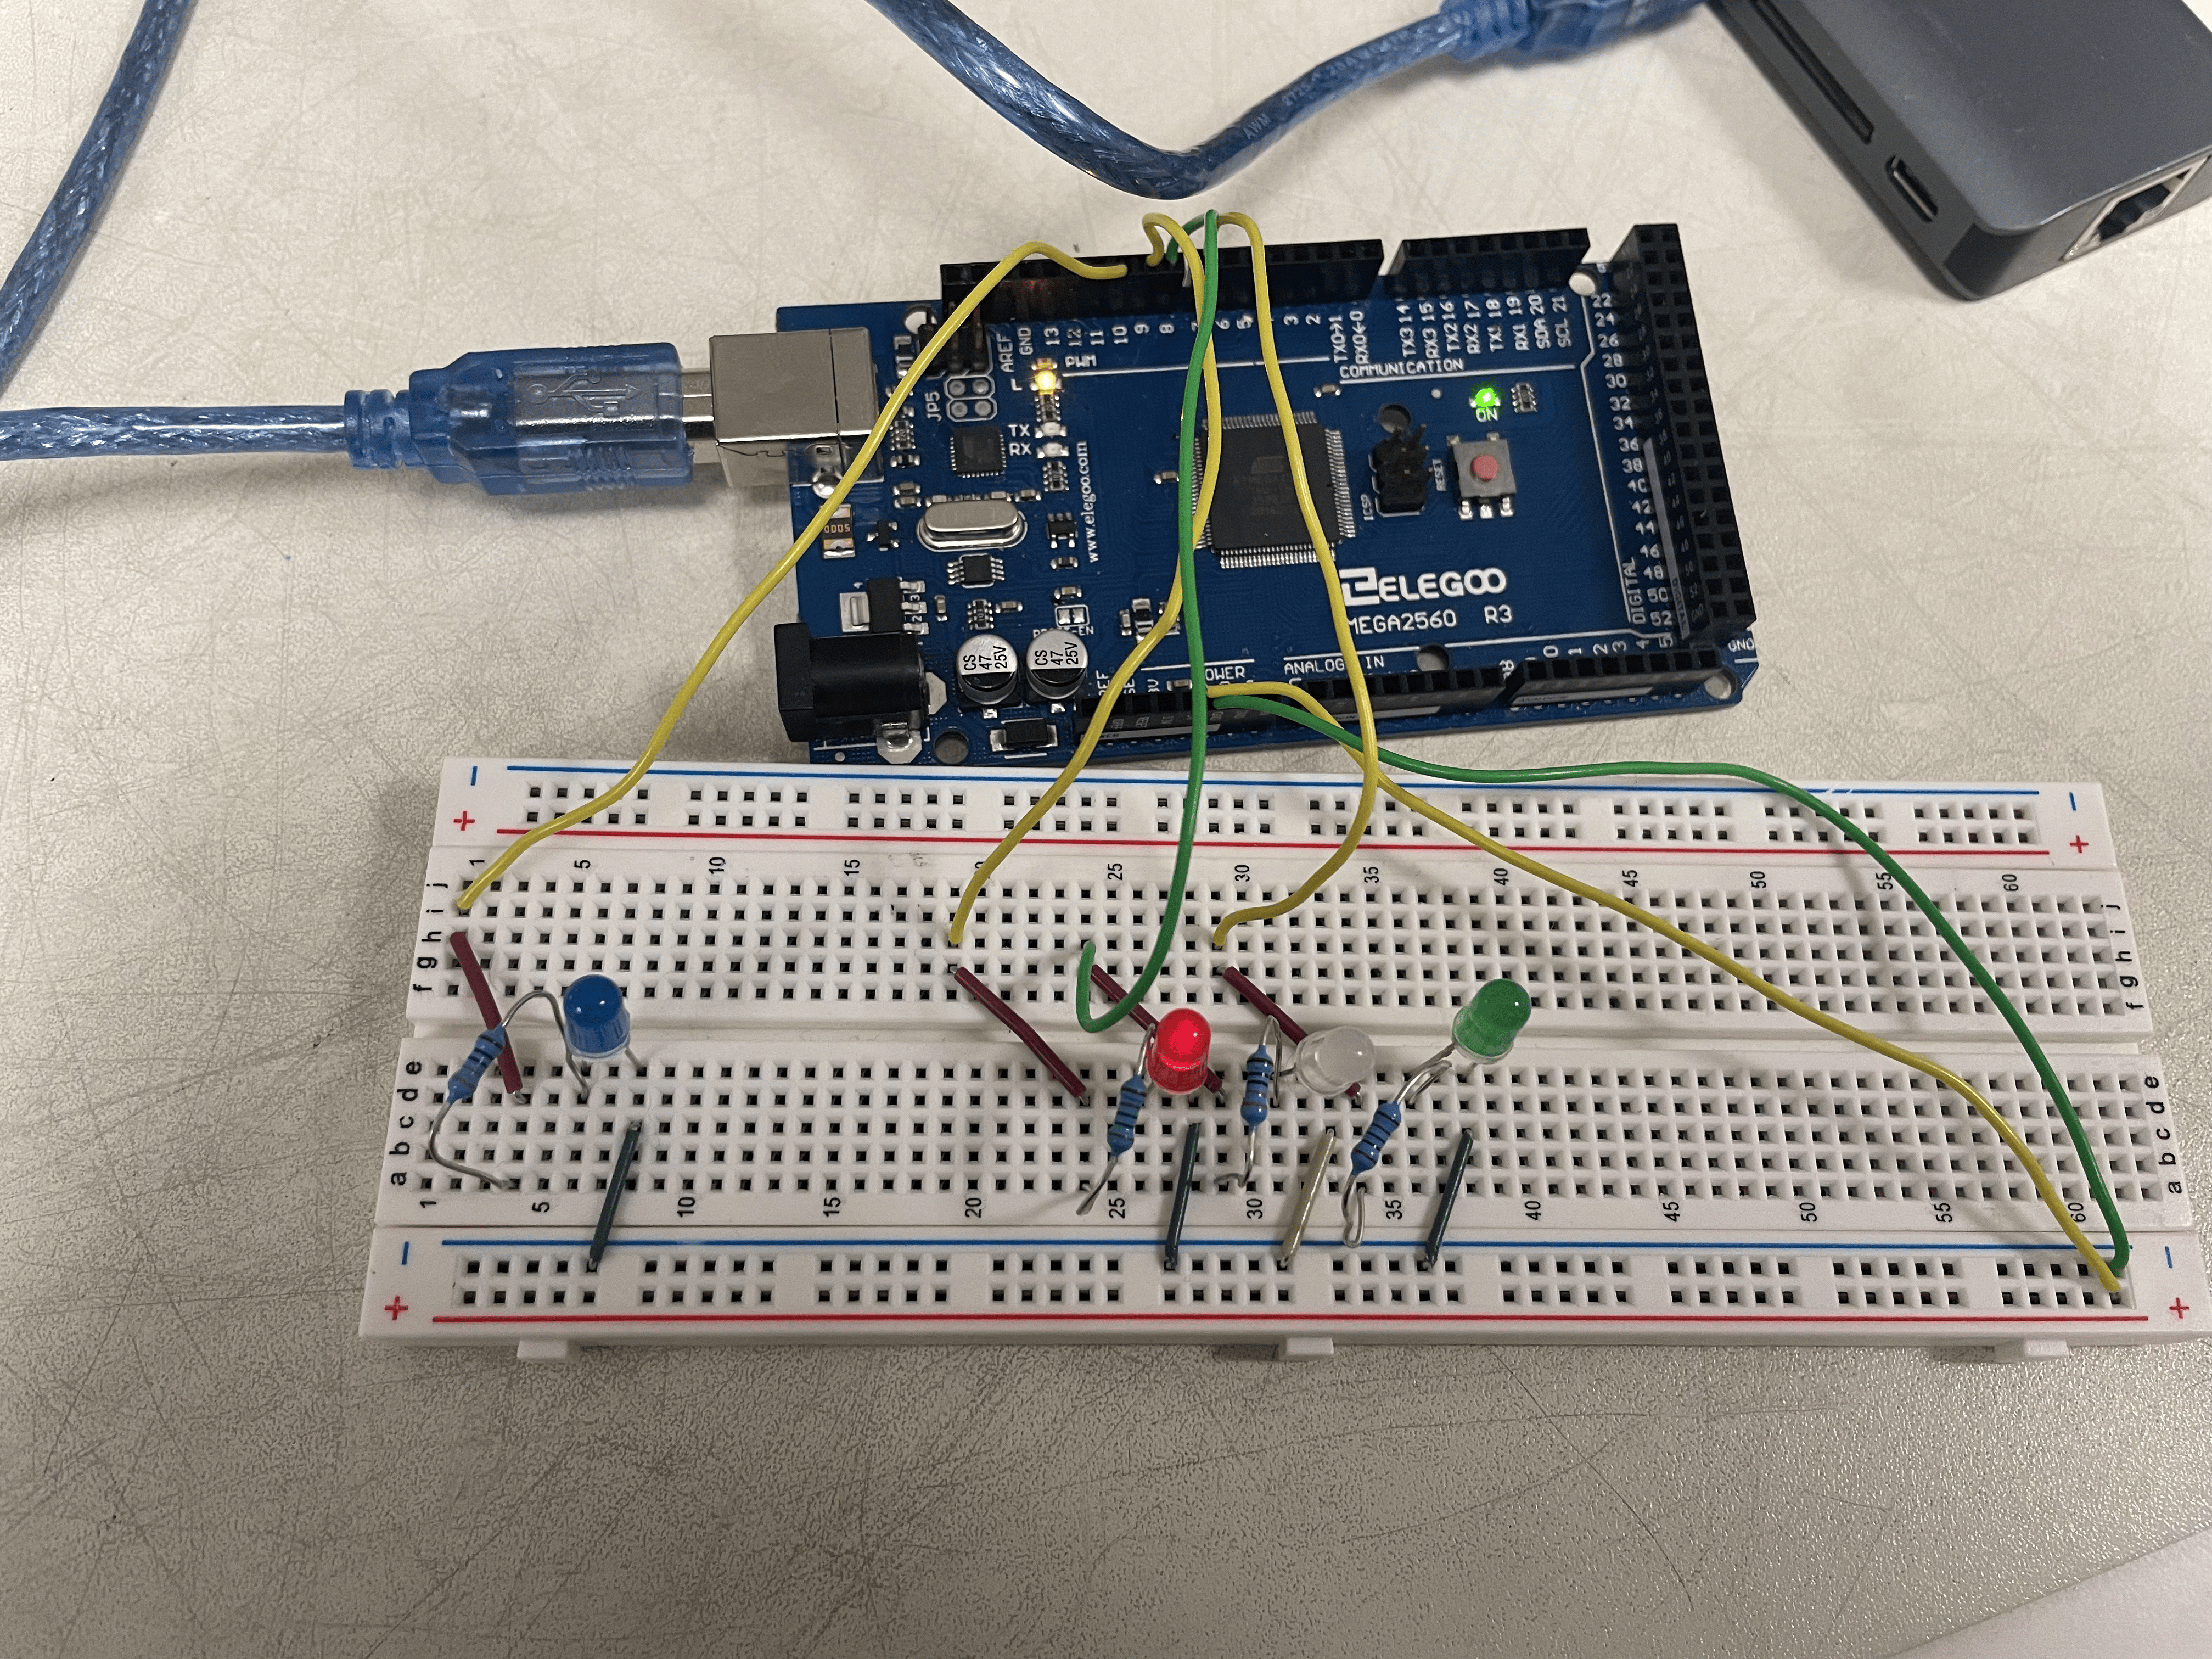
\includegraphics[width=0.28\linewidth]{red.jpg}
            \\
            State 0: Lights off.&
            State 1: Red light.
            \\
        \hline
            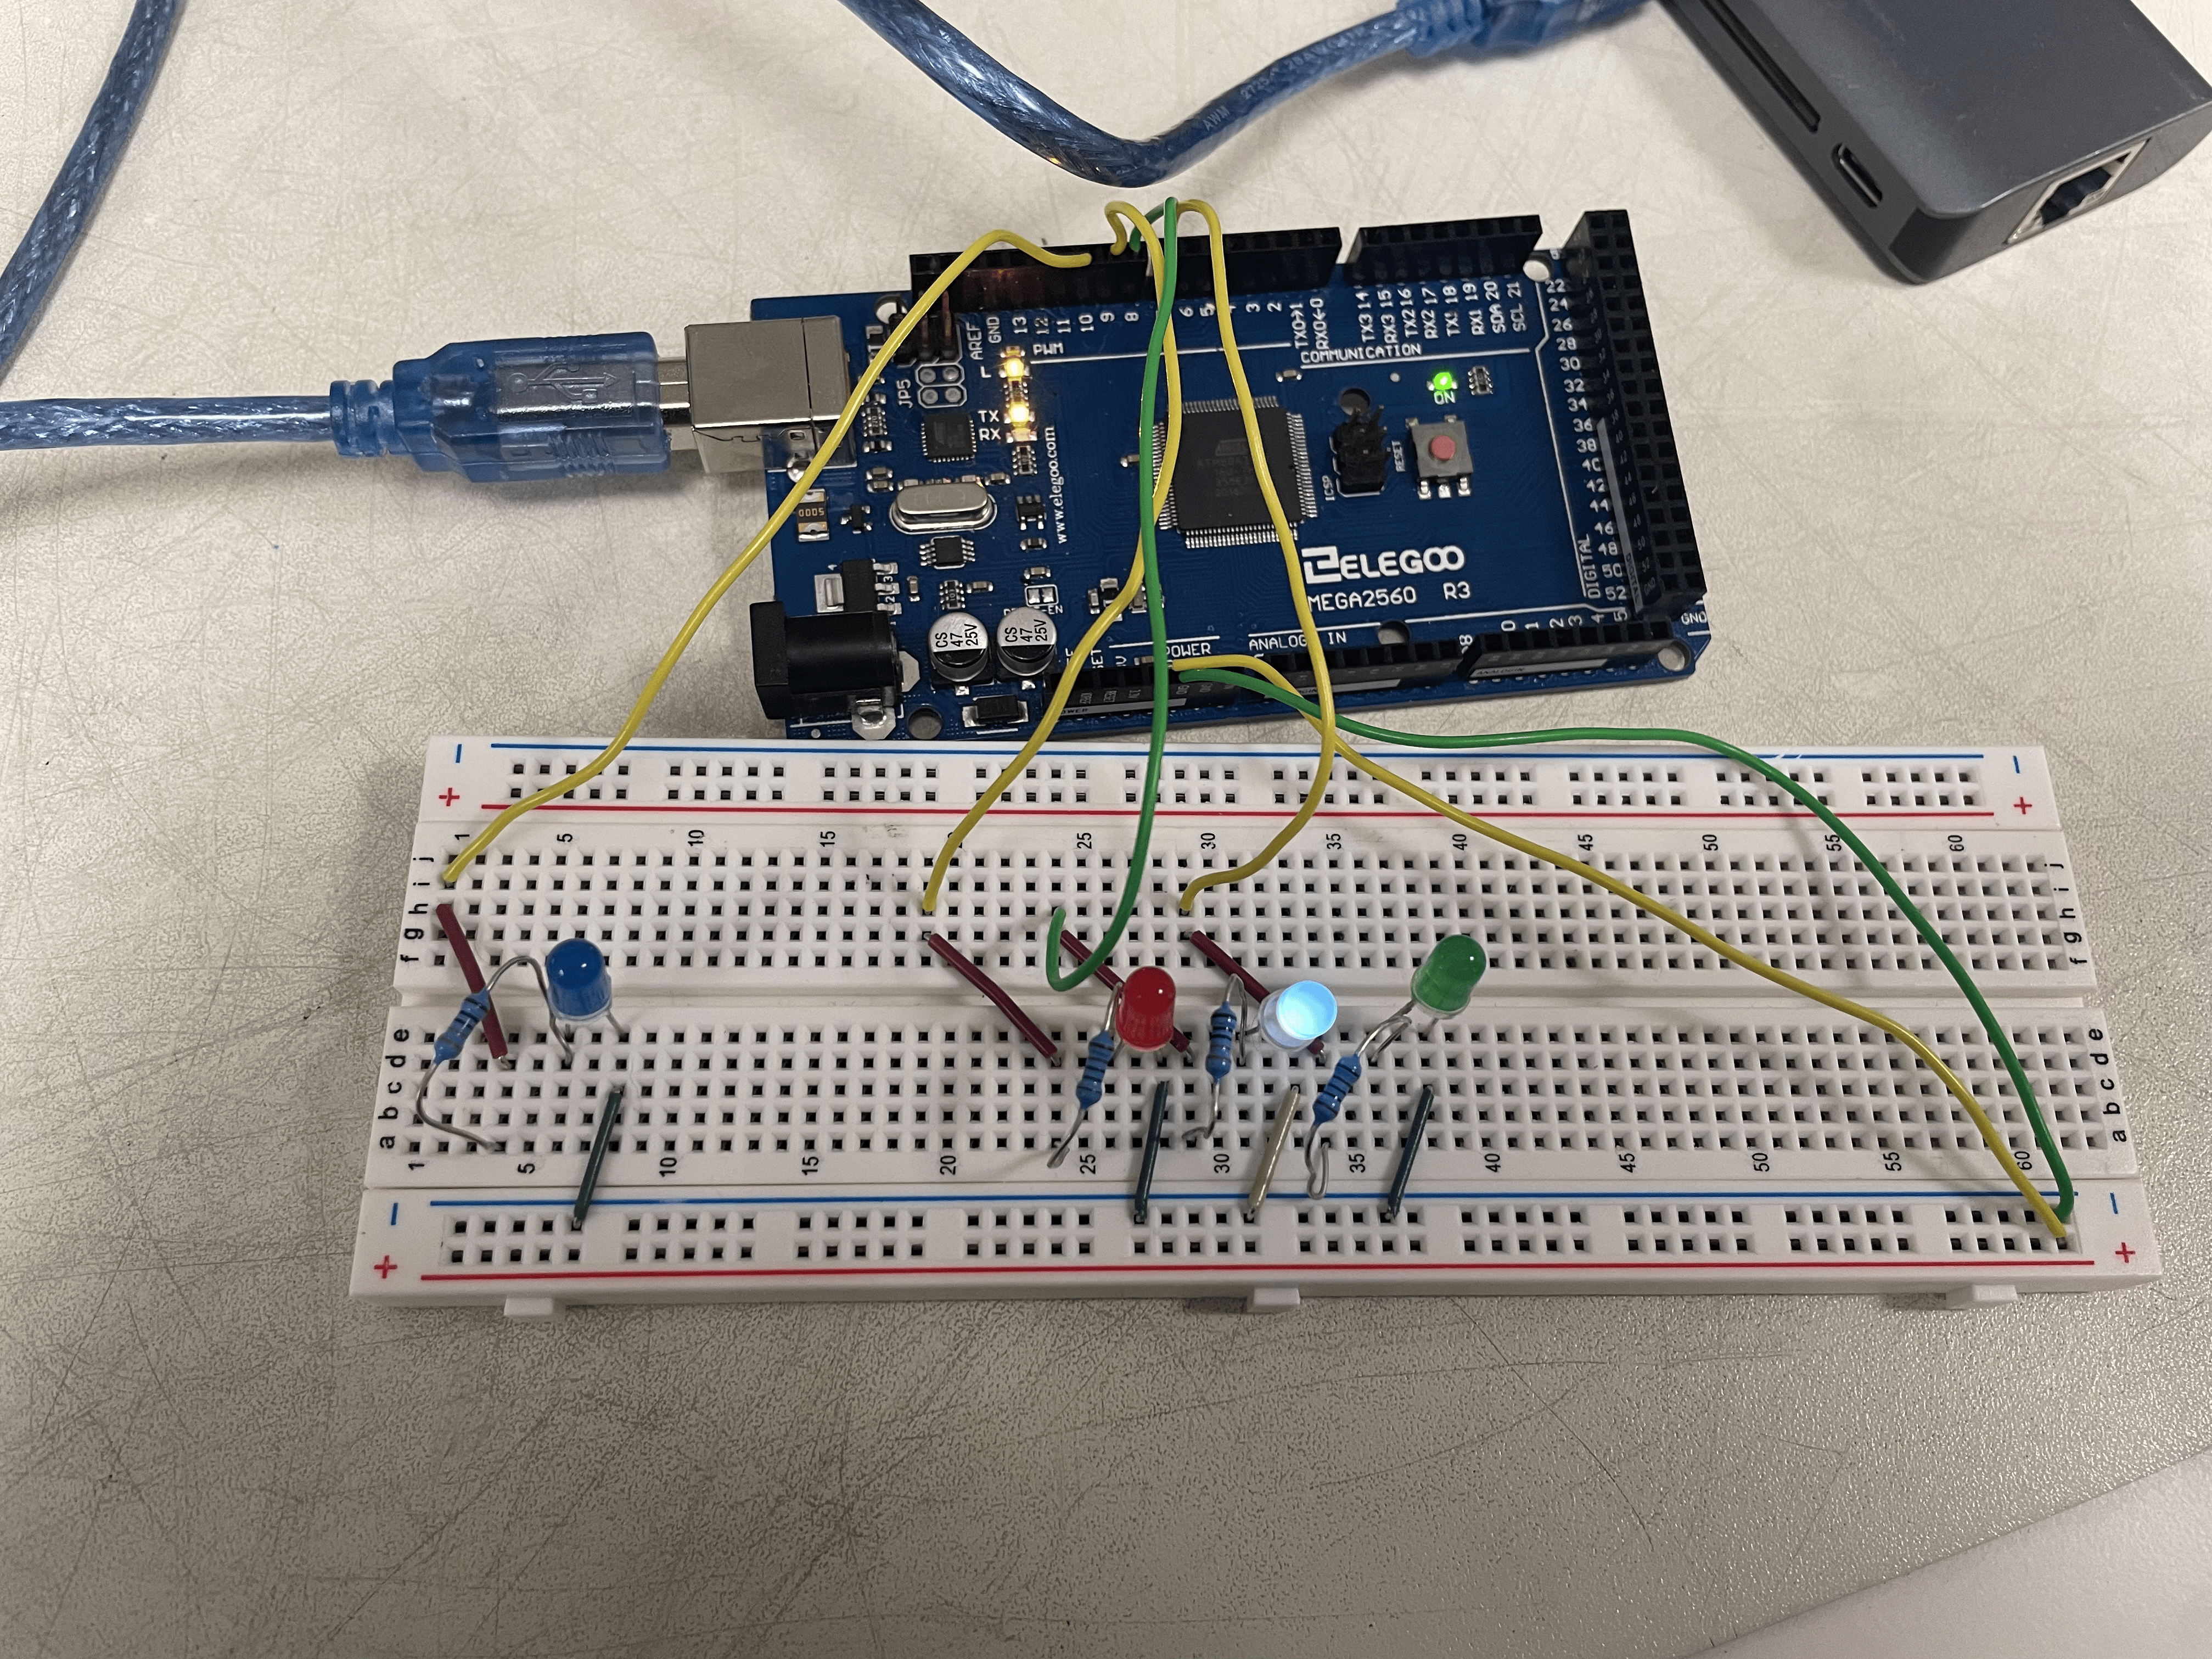
\includegraphics[width=0.28\linewidth]{yellow.jpg}&
            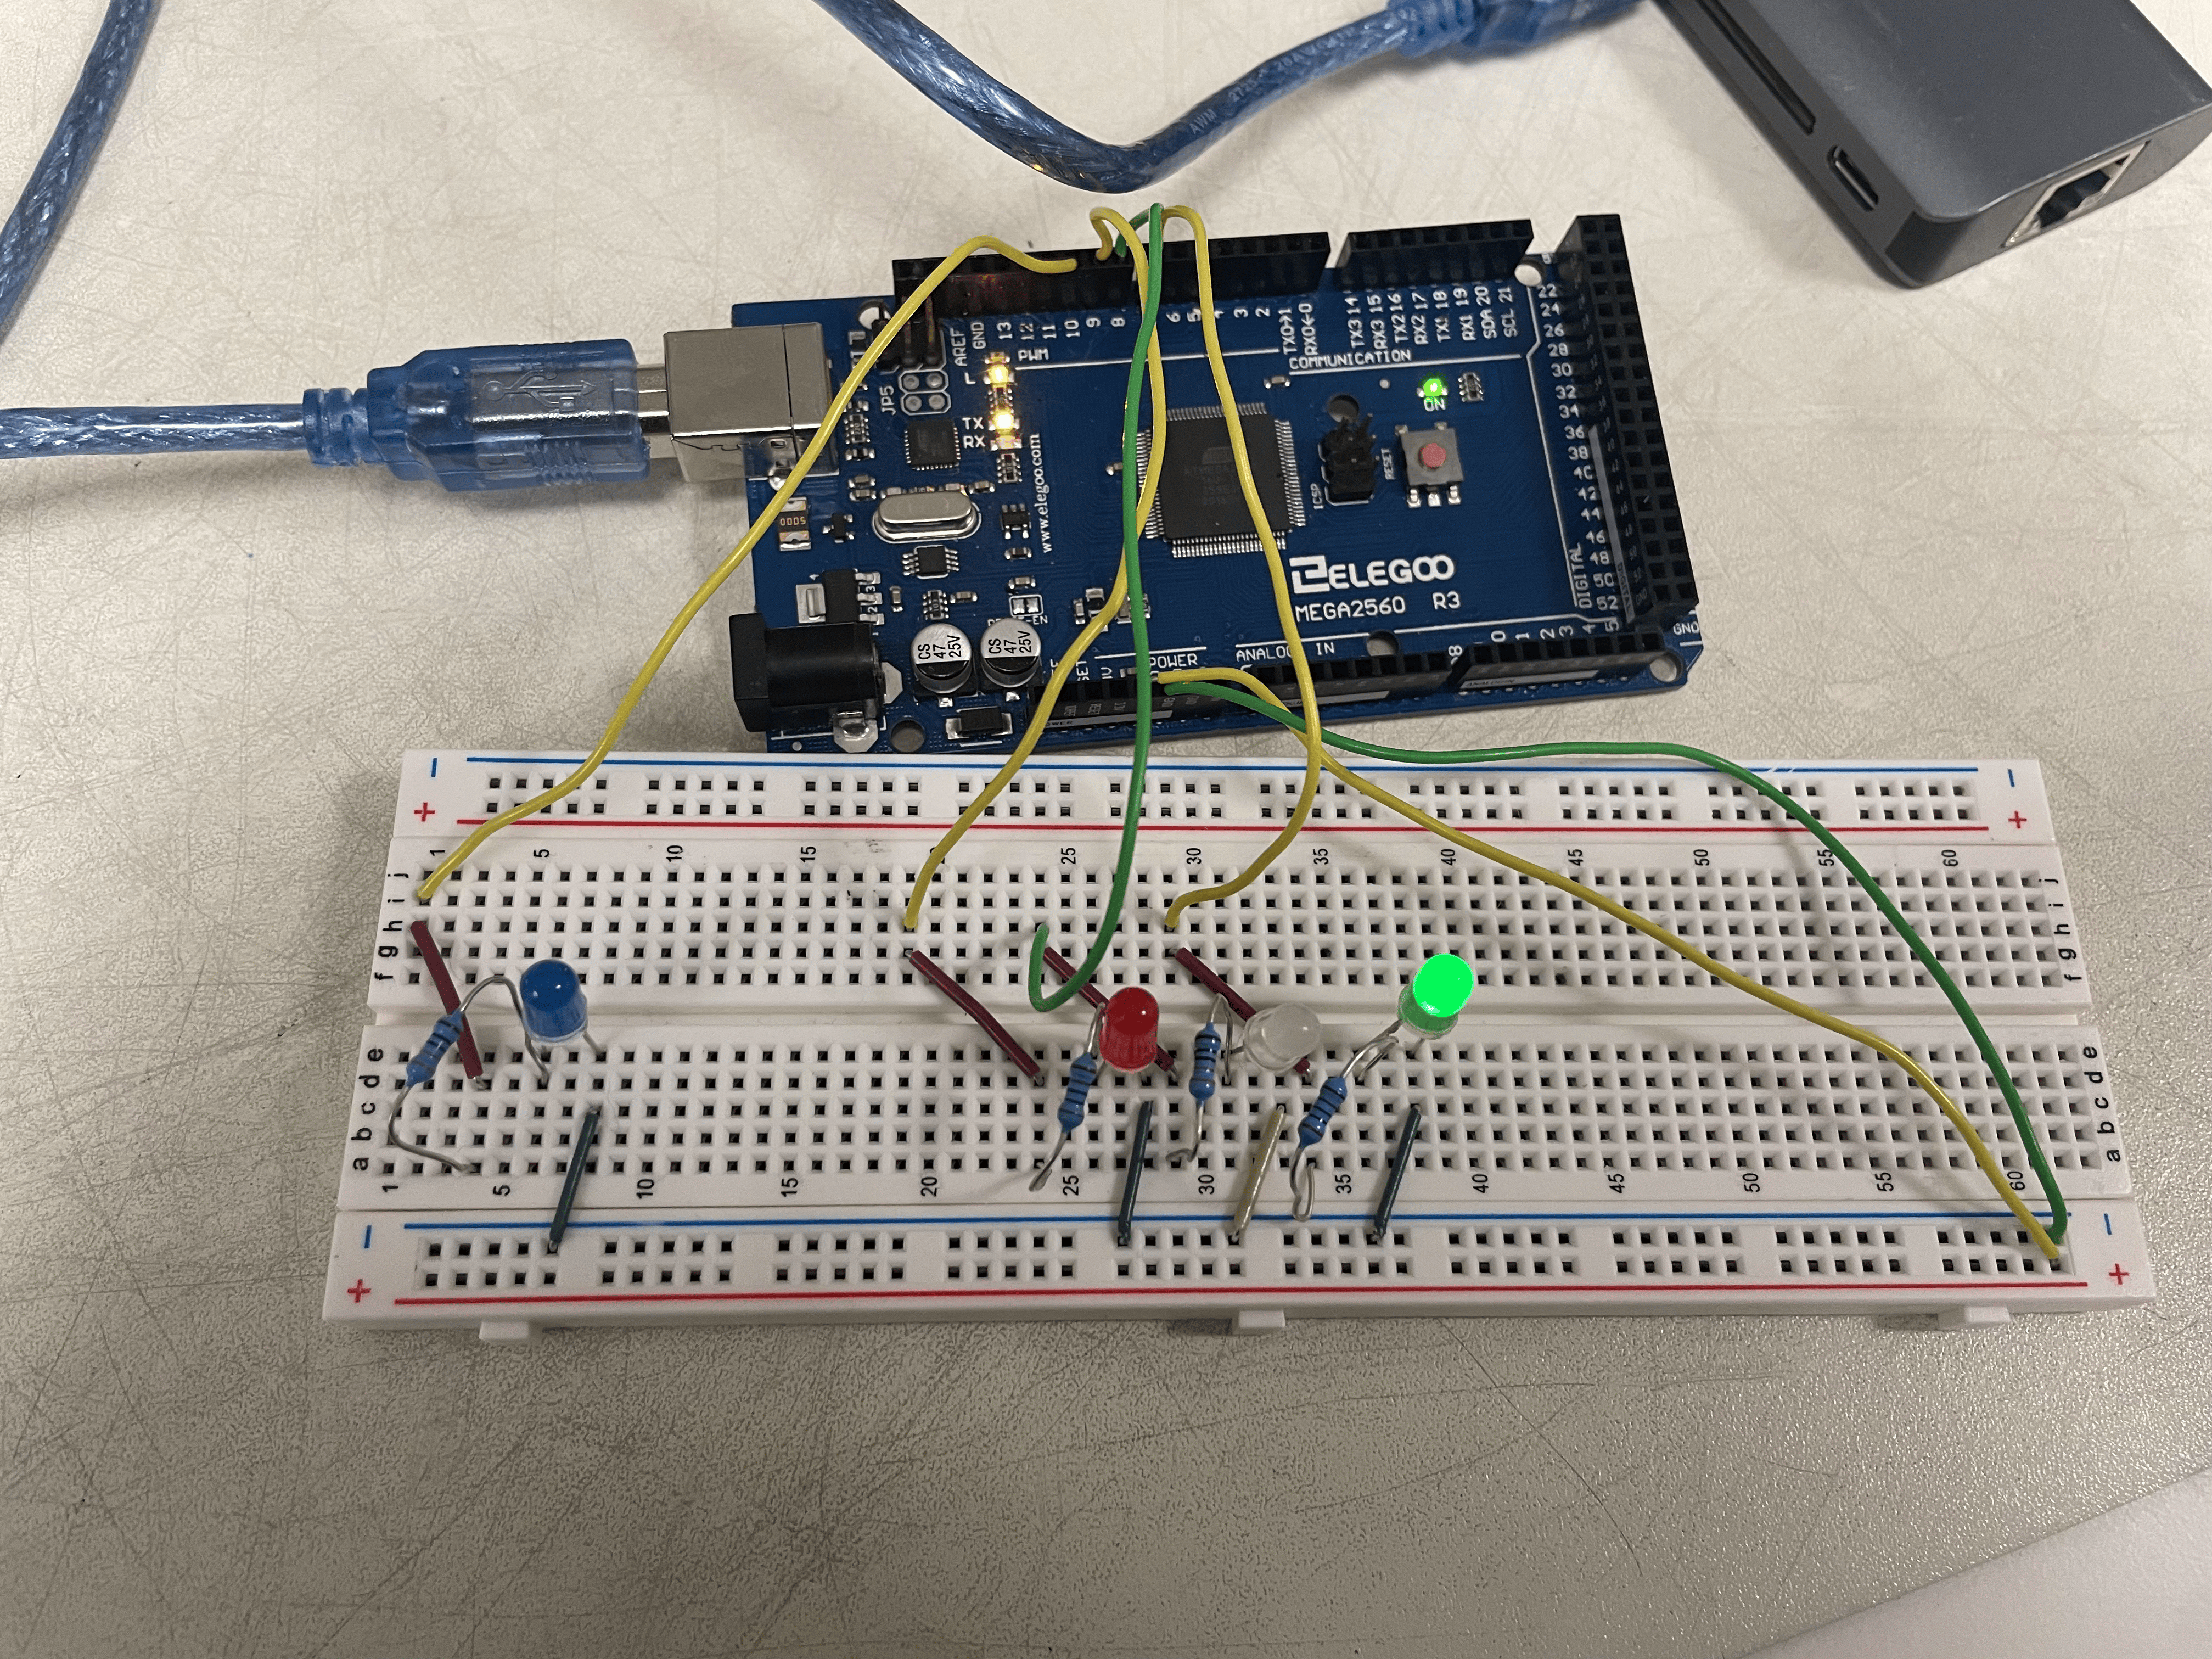
\includegraphics[width=0.28\linewidth]{green.jpg} 
            \\
            State 2: Yellow light.&
            State 3: Green light.
            \\
        \hline
    \end{tabular}
    \caption{The various light configurations that result from the circuit.}
    \label{tab:light-configs}
\end{table}

\subsection{Code}

\subsubsection{Part 1}

The code for part 1 was made with Arduino IDE, and was designed using modulus. We took a counter that increments at every button press, and the result of the counter value \% 4 would dictate the state of the lights in a switch case (1 to red, 2 to yellow, 3 to green, and 0 to none).

\subsubsection{Part 2}

The code for part 2 is similar, we replaced all calls to the Arduino library. We utilize the port registers to operate on the LEDs and read in the button. For example, the green LED, connected to port 7 is represented as 'on' with the binary expression `0b00010000`.
 
View code on \href{https://github.com/jrkre/cpe-301}{GitHub}.


\end{document}